\documentclass[a4paper, 12pt]{report}


\usepackage[utf8]{inputenc}
\usepackage[T1]{fontenc}
\usepackage[spanish]{babel} 
\usepackage{graphicx}
\usepackage{amsmath}
\usepackage{amssymb}
\usepackage{mathtools}
\usepackage{amsthm}
\usepackage{bbm}
%\usepackage[shortlabels]{enumitem}
\usepackage{enumerate}
\usepackage{array,tabularx}
\usepackage{float}
\usepackage{wrapfig}
\usepackage[export]{adjustbox}
\usepackage[rightcaption]{sidecap}
\usepackage{multirow}
\usepackage{subfig}
\usepackage{capt-of}
\usepackage{captdef}
\usepackage{color}
\usepackage{ebproof}
\usepackage{soul}
\usepackage{hyperref}
\usepackage{ebproof}
\usepackage{stmaryrd}
\usepackage{fullpage}
\usepackage{xcolor}

\newcommand{\Ra}{\Rightarrow}
\newcommand{\ra}{\rightarrow}
\newcommand{\N}{\mathbb{N}}
\newcommand{\R}{\mathbb{R}}
\newcommand{\te}{\text}
\newcommand{\Lra}{\Leftrightarrow}
\newcommand{\lra}{\leftrightarrow}


\newtheorem{teorema}{Teorema}[section]
\newtheorem{lema}[teorema]{Lema}
\newtheorem{corolario}[teorema]{Corolario}
\newtheorem{prop}[teorema]{Proposición}
\newtheorem*{prop*}{Proposición}

\theoremstyle{definition}
\newtheorem{definicion}[teorema]{Definición}
\newtheorem*{definicion*}{Def}
\newtheorem{obs}[teorema]{Observación}
\newtheorem*{ejemplo*}{Ejemplo}
\newtheorem*{ejemplos*}{Ejemplos}
\newtheorem*{notacion}{Notación}
\newtheorem{ejercicio}{Ejercicio}[section]

\begin{document}

\tableofcontents

\chapter{Elementos de lógica de primer orden}

La lógica de primer orden es un marco de formalización de la matemática. Permite definir precisamente nociones como la de teorema y demostración. Esto además de su interés intrínseco, abre la puerta a la verificación automática de demostraciones, lo cual permite utilizar computadoras para verificar todos los detalles de una prueba. Como la denominación <<de primer orden>> sugiere, hay otros tipos de lógicas de mayor orden, pero cabe aclarar que no son indispensables para formalizar la matemática.

\section{Introducción}

El objetivo de este capítulo es introducir algunas nociones básicas de lógica de primer orden y de teorías de primer orden. Sin embargo, antes de eso se presentan algunos conceptos centrales que no suelen aparecer en otras áreas de la matemática, como son la mateteoría y la definición por inducción estructural.

\subsection{Metateoría y teoría}

Es común que al comenzar a estudiar lógica uno tenga la expectativa de justificar la matemática a partir de razonamientos más elementales, sin hacer ninguna hipótesis. Está bueno desde ya dejar claro que eso no se puede (o no parece poderse). Como se verá en seguida, ya para definir el lenguaje de la matemática se necesitan nociones matemáticas al menos tan complejas como los números naturales. En lugar de estudiar la matemática desde afuera, vamos a estudiarla usando la misma matemática como herramienta. Un cierto nivel de circularidad parece inevitable para poder decir cosas precisas y no triviales.

Con ese fin de estudiar formalmente la matemática usando la misma matemática, para no caer en paradojas se introduce la distinción entre \textbf{metateoría} y \textbf{teoría}. La metateoría y la teoría son dos niveles distintos de matemática: la que se usa como herramienta y la que es estudiada como un objeto, respectivamente. Es decir, la teoría es la matemática que está siendo estudiada formalmente y la metateoría consiste en los razonamientos matemáticos que se hacen sobre la teoría. Dentro de la metateoría, la teoría consistirá en objetos definidos matemáticamente sobre los que se razonará matemáticamente de forma usual. La gracia es que la teoría modelará el mismo razonamiento de la metateoría. Si se quiere, se puede pensar que la metateoría consiste en razonamientos matemáticos primitivos, con los cuales definimos la teoría como un objeto matemático formal que modela el mismo razonamiento matemático.

Si bien es necesario partir de una metateoría, la buena noticia es que en esa metateoría va a ser muy elemental. Va a estar al mismo nivel que las operaciones aritméticas que se aprenden en la escuela. Por una parte, los objetos con los que trabajaremos serán todos objetos finitos. Por otra parte, solo requeriremos operaciones definidas por reglas precisas y que terminan en una cantidad finita de pasos. En otras palabras, sin ambigüedad, con una cantidad finita de lápiz y papel y en tiempo finito, podremos verificar la correctitud de lo que hayamos hecho. Equivalentemente, se puede escribir programas que con suficiente memoria y suficiente tiempo de ejecución, realizan la verificación de forma automática.

\subsection{Definición por inducción estructural}\label{sec-IndEstr}

La inducción estructural es una forma de definir conjuntos de objetos finitos recursivos, es decir que contienen otros objetos del mismo tipo más pequeños. Cada definición por inducción estructural está dada por un conjunto finito de reglas base y reglas inductivas. Tener un conjunto de objetos definido por inducción estructural nos da un principio de demostración por inducción y un principio de definición de funciones por recursión, similares a los de $\N$. El ejemplo canónico de definición por recursión en $\N$ es el factorial:
\begin{enumerate}
	\item $0! = 1$.
	\item $(n+1)! = (n+1)n!$ para todo $n\in\N$.
\end{enumerate}

 Tanto el lenguaje de la lógica de primer orden como las demostraciones en sí serán definidos por inducción estructural (con muchas reglas).

Las reglas de base dan directamente elementos que pertenecen al conjunto, mientras que las reglas inductivas permiten construir elementos a partir de otros previamente construidos.
Dado un conjunto de reglas de base y reglas inductivas, el conjunto que definen es el de todos los objetos que pueden construirse aplicando las reglas finitas veces.
Veamos algunos ejemplos, junto con sus principios de inducción y recursión.

\subsubsection{Enteros de Peano}
Este es el ejemplo más sencillo de conjunto definido por inducción.
\begin{definicion*}
	Definimos por inducción al conjunto \texttt{Nat} en base a las siguientes dos reglas:
	\begin{enumerate}
		\item \textbf{RB)} $Z\in \mathtt{Nat}$.
		\item \textbf{RI)} Si $n\in\mathtt{Nat}$, entonces $S(n)\in\mathtt{Nat}$.
	\end{enumerate}
\end{definicion*}

La primera regla es de base y la segunda es inductiva. Los elementos de \texttt{Nat} son $Z$, $S(Z)$, $S(S(Z))$, etc. Es importante aclarar que los elementos de $\mathtt{Nat}$ son todos los que se pueden construir mediante finitas aplicaciones de las reglas y ningún otro. El nombre \texttt{Nat} es porque representan a los números naturales, con $Z\sim 0$, $S(Z)\sim 1$, $S(S(Z))\sim 2$, etc.
Enunciemos el principio de inducción y el principio de recursión para $\mathtt{Nat}$.
\begin{prop*}[Inducción de $\mathtt{Nat}$]
	
	Sea $\phi(x)$ una propiedad. Si:
	\begin{enumerate}
		\item $\phi(Z)$.
		\item Para todo $n\in\mathtt{Nat}$, si $\phi(n)$ entonces $\phi(S(n))$.
	\end{enumerate}
	Entonces $\forall n\in\mathtt{Nat},~\phi(n)$.
\end{prop*}
Es decir, si probamos que una propiedad se cumple para $Z$ y además asumiendo que se cumple para $n\in\mathtt{Nat}$ probamos que también se cumple para $S(n)$, tenemos que se cumple para todo $n\in\mathtt{Nat}$.

\begin{prop*}[Recursión de $\mathtt{Nat}$]
	Sea $X$ un conjunto. Queremos definir una función $f:\mathtt{Nat}\to X$. Si:
	\begin{enumerate}
		\item Definimos $f(Z)$.
		\item Para cada $n\in\mathtt{Nat}$, asumiendo que $f(n)$ está definido, definimos $f(S(n))$.
	\end{enumerate}
	Entonces $f$ queda definida en todo $\mathtt{Nat}$.
\end{prop*}
A modo de ejemplo, podemos definir la correspondencia $\phi:\mathtt{Nat}\to\N$:
\begin{enumerate}
	\item $\phi(Z) = 0$.
	\item $\phi(S(n)) = \phi(n) + 1$ para todo $n\in\mathtt{Nat}$.
\end{enumerate}
Con esas dos reglas la función queda definida. Para calcularla aplicamos la regla 2 reiteradamente hasta llegar al caso de la regla 1. Por ejemplo:
$$ \phi(S(S(S(Z)))) = \phi(S(S(Z))) + 1 = \phi(S(Z)) + 2 =
\phi(Z) + 3 = 0 + 3 = 3
$$

Por otra parte, se puede definir una función de varias variables haciendo recursión en uno de los argumentos y dejando a los otros como parámetros. Definimos la suma de dos elementos de $\mathtt{Nat}$ dejando al primer elemento como parámetro y haciendo recursión en el segundo. En este caso estamos definiendo $+:\mathtt{Nat}\times\mathtt{Nat}\to\mathtt{Nat}$, aunque como es usual, en lugar de escribir $+(n,m)$ escribiremos $n+m$. La definición es la siguiente:
\begin{enumerate}
	\item $n + Z = n$.
	\item $n + S(p) = S(n+p)$ para todo $p\in\mathtt{Nat}$.
\end{enumerate}
En el segundo caso estamos definiendo $n+S(p)$ asumiendo que $n+p$ ya está definido. A modo de ejemplo (pintando el parámetro de azul):

$$ \textcolor{blue}{S(S(Z))} + S(S(Z)) = S(\textcolor{blue}{S(S(Z))} + S(Z)) = S(S(\textcolor{blue}{S(S(Z))} + Z)) = S(S(\textcolor{blue}{S(S(Z))}))
$$
donde las primeras dos igualdades son por la regla 2 y la tercera es por la regla 1.

Vamos ahora a demostrar una propiedad de la suma usando el principio de inducción de \texttt{Nat}. Por definición tenemos que $Z$ es neutro a derecha, es decir que $n+Z=N$ para todo $n\in\mathtt{Nat}$. Probaremos por inducción que también es neutro a izquierda.

\begin{prop*}
	Para todo $n\in\mathtt{Nat}$ se cumple que $Z+n=n$.
\end{prop*}
\begin{proof}
	Usamos el principio de inducción de \texttt{Nat} con $\phi(x)~\equiv~ Z+x=x$. Para el paso base hay que probar $\phi(Z)$, es decir $Z+Z=Z$. Se cumple por definición de la suma. Continuamos con el paso inductivo.
	
	Sea $n\in\mathtt{Nat}$. La hipótesis es $\phi(n)$, o sea $Z+n=n$, mientras que la tesis es $\phi(S(n))$, lo cual se traduce a $Z+S(n)=S(n)$. Se concluye usando la definición de suma y la hipótesis inductiva: $Z+S(n) = S(Z+n) = S(n)$.
\end{proof}
\begin{ejercicio}
	Demostrar las siguientes propiedades de la suma. Se recomienda elegir un sumando para hacer inducción y dejar los otros como parámetros.
	\begin{enumerate}
		\item $S(n)+m = S(n+m)$.
		\item $m+n = m+n$.
		\item $(m+n)+p = m+(n+p)$.
	\end{enumerate}
	
\end{ejercicio}
\begin{ejercicio}
	Definir el producto de $\mathtt{Nat}$ por inducción en el segundo argumento y utilizando la suma ya definida (en la sección siguiente hay un ejemplo de función recursiva que usa otra anterior). Demostrar algunas propiedades análogamente al ejercicio anterior (si se quiere probar la asociativa, probablemente se necesite la distributiva antes).
\end{ejercicio}

\subsubsection{Listas finitas de naturales}

Vamos a definir por inducción un nuevo conjunto dado por listas finitas de números de $\N$. Lo que aporta este ejemplo es que la regla inductiva tiene un parámetro aparte de la lista previamente construida.

\begin{definicion*}
	Definimos por inducción al conjunto \texttt{List} con las siguientes reglas:
	\begin{enumerate}
		\item \textbf{RB)} $[]\in\mathtt{List}$.
		\item \textbf{RI)} Si $n\in\N$ y $l\in\mathtt{List}$, entonces $n:l\in\mathtt{List}$.
	\end{enumerate}
\end{definicion*}
La lista $[]$ es la lista vacía. Un ejemplo de lista no vacía es $1:2:3:[]$. El principio de inducción y el de recursión para este  conjunto son los siguientes.
\begin{prop*}[Inducción de $\mathtt{List}$]
	
	Sea $\phi(x)$ una propiedad. Si:
	\begin{enumerate}
		\item $\phi([])$.
		\item Para toda $l\in\mathtt{List}$ y todo $n\in\N$, si $\phi(l)$, entonces $\phi(n:l)$.
	\end{enumerate}
	Entonces $\forall l\in\mathtt{List},~\phi(l)$.
\end{prop*}
\begin{prop*}[Recursión de $\mathtt{List}$]
	Sea $X$ un conjunto. Queremos definir una función $f:\mathtt{List}\to X$. Si:
	\begin{enumerate}
		\item Definimos $f([])$.
		\item Para cada $l\in\mathtt{List}$ y $n\in\N$, asumiendo que $f(l)$ está definido, definimos $f(n:l)$.
	\end{enumerate}
	Entonces $f$ queda definida en todo $\mathtt{List}$.
\end{prop*}
En este caso con el principio de recursión se puede definir de forma trivial funciones que no parecen tan obvias. Dados $n\in\N$ y $l\in\mathtt{List}$, la lista que resulta al agregarlo en primer lugar es $n:l$. ¿Y si queremos agregarlo en el último lugar? Para esto definimos una función $f:\N\times\mathtt{List}\to\mathtt{List}$, de modo que $f(n,l)$ sea la lista que resulta al agregar $n$ en el último lugar de $l$. Definimos $f$ por inducción en el segundo argumento.
\begin{enumerate}
	\item $f(n,[]) = n:[]$.
	\item $f(n,x:l) = x:(f(n,l))$.
\end{enumerate}
Es muy interesante (a mi parecer) que con eso el problema esté resuelto. Parece que no hubieramos hecho nada, pero por el principio de recursión ya está. El razonamiento es el siguiente. En el caso de que la lista es vacía, claramente hay que retornar la lista que solamente tiene el elemento que queremos agregar al final. Cuando la lista es $x:l$, por el principio de recursión ya sabemos insertar $n$ al final de la lista $l$: el  resultado es $f(n,l)$. Por lo tanto, el resultado de insertar $n$ al final de la lista $x:l$ no es más que $x:(f(n,l))$.

Definimos ahora una función $r:\mathtt{List}\to\mathtt{List}$ que retorna la lista invertida.
\begin{enumerate}
	\item $r([]) = []$.
	\item $r(n:l) = f(n,r(l))$.
\end{enumerate}

\begin{ejercicio}
	\begin{enumerate}
		\item Interpretar la definición recursiva de la función $r$, como se hizo con $f$.
		\item Evaluar paso a paso $r(1:2:3:[])$.
		\item Demostrar por inducción que $\forall l\in\mathtt{List},~r(r(l))=l$. Sugerencia: conjeturar y demostrar por inducción el resultado de $r(f(x,l))$.
	\end{enumerate}
\end{ejercicio}
\begin{ejercicio}
	Definir por recursión  una función que duplique todas las entradas de una lista, una función que sume todas las entradas de una lista, conjeturar una fórmula para el resultado de la composición y demostrarla por inducción.
\end{ejercicio}

\subsubsection{Árboles y múltiples reglas}

Veamos por último un ejemplo en el que el conjunto tiene estructura de árbol y además hay múltiples reglas inductivas. También pueden haber múltiples reglas de base, como ocurrirá varias veces más adelante. Definimos artificialmente el conjunto $\mathtt{C}$ con las siguientes reglas.
\begin{enumerate}
	\item \textbf{RB)} $\square\in C$.
	\item \textbf{RI)} Si $x\in C$, entonces $\circ x\in C$.
	\item \textbf{RI)} Si $x\in C$ y $y\in C$, entonces $x\triangle y\in C$.
\end{enumerate}
Decimos que tiene estructura de árbol por la regla 3. El elemento $x\triangle y$ se puede pensar como una bifurcación con rama izquierda $x$ y rama derecha $y$. Por otra parte, los círculos son ramas sin bifurcación y los cuadrados son hojas (en seguida hay dos ejemplos). Notar que a veces se necesitan paréntesis para que no sea ambiguo. A modo de ejemplo, $(\circ \square)\triangle\square$ y $\circ(\square\triangle\square)$ son elementos distintos, con las siguientes representaciones como árboles.

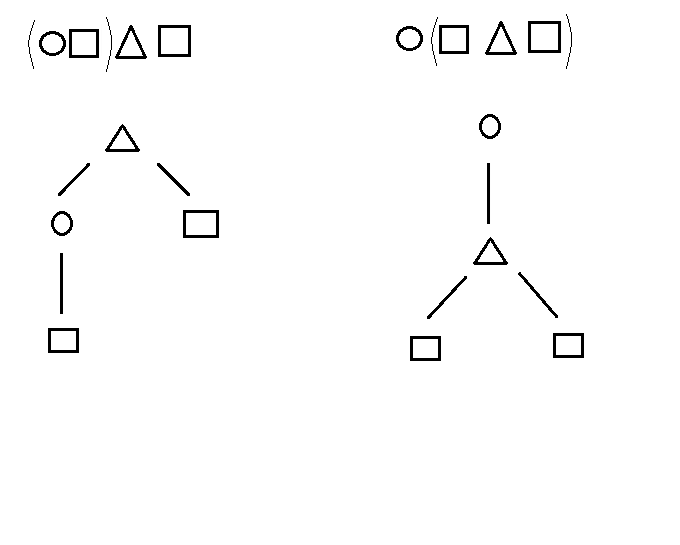
\includegraphics[scale=0.6]{figPaint.png}

El principio de inducción y el de recursión son los siguientes.
\begin{prop*}[Inducción de $\mathtt{C}$]
	
	Sea $\phi(x)$ una propiedad. Si:
	\begin{enumerate}
		\item $\phi(\square)$.
		\item Para todo $x\in\mathtt{C}$, si $\phi(x)$ entonces $\phi(\circ x)$.
		\item Para todos $x,y\in\mathtt{C}$, si $\phi(x)$ y $\phi(y)$, entonces $\phi(x\triangle y)$.	\end{enumerate}
	Entonces $\forall x\in\mathtt{C},~\phi(x)$.
\end{prop*}
\begin{prop*}[Recursión de $\mathtt{C}$]
	Sea $X$ un conjunto. Queremos definir una función \linebreak$f:\mathtt{C}\to X$. Si:
	\begin{enumerate}
		\item Definimos $f(\square)$.
		\item Para cada $x\in\mathtt{C}$, asumiendo que $f(x)$ está definido, definimos $f(\circ x)$.
		\item Para cada par $x,y\in\mathtt{C}$, asumiendo que $f(x)$ y $f(y)$ están definidos, definimos $f(x\triangle y)$.
	\end{enumerate}
	Entonces $f$ queda definida en todo $\mathtt{C}$.
\end{prop*}

\begin{ejercicio}
	\begin{enumerate}
		\item Dibujar el árbol de $(\circ\circ\square)\triangle(\square\triangle\circ\square)$.
		\item Definir por recursión una función $c:C\to\N$ tal que $c(x)$ sea la cantidad de cuadrados que aparecen en $x$ y aplicarla paso a paso al elemento de la parte 1.
		\item Demostrar por inducción que $\forall x\in C,~c(x)\geq 1$.
	\end{enumerate}
\end{ejercicio}

\section{Lenguajes de primer orden}

Comenzaremos a definir los elementos sintácticos de la lógica de primer orden. Un resultado de esto será tener una noción formal de enunciado matemático. Recordar que no vamos a intentar formalizar la matemática desde fuera, sino que definiremos matemáticamente <<objetos matemáticos que modelan al lenguaje y razonamiento matemático>> y razonaremos matemáticamente de modo usual sobre esos objetos. Usaremos con soltura las técnicas de definición y demostración introducidas en la sección \ref{sec-IndEstr}.

\subsection{Vocabularios}

Los lenguajes de primer orden están parametrizados por un vocabulario. Esto es necesario porque hay elementos sintácticos específicos de distintas teorías. Por ejemplo, los símbolos $0,+,\times,\leq$ tienen sentido en la teoría de cuerpo ordenado pero no en la teoría de conjuntos. Por otra parte, con $\varnothing,\cup,\mathcal{P},\subseteq$ es al revés.

\begin{definicion}[Vocabulario]
	Un vocabulario $\mathtt{V}$ está dado por:
	\begin{itemize}
		\item Un conjunto de símbolos de función $\mathtt{F}$, denotadas por ejemplo $f$, $g$, etc.
		\item Un conjunto disjunto a $\mathtt{F}$ de símbolos de predicado $\mathtt{P}$, denotadas a veces $p$, $q$, etc.
		\item Una función de aridad $\#:\mathtt{F}\cup\mathtt{P}\to\N$.
	\end{itemize}
	Decimos que un símbolo de función $f$ es de aridad $k$ si $\#(f)=k$ (ídem con predicados).
\end{definicion}
Los símbolos de función representan operaciones primitivas o constantes. La aridad indica la cantidad de operandos (las constantes son el caso particular de aridad nula). Los símbolos de predicado representan relaciones o propiedades primitivas. En caso de aridad 1 es una propiedad, sino es una relación que vincula esa cantidad de elementos. A modo de ejemplos intuitivos:
\begin{itemize}
	\item $0$, $\varnothing$ son símbolos de función de aridad 0.
	\item $\mathcal{P}$ es un símbolo de función de aridad 1 (conjunto potencia).
	\item $+,\times,\cup$ son símbolos de función de aridad 2.
	\item $pos$ es un símbolo de predicado de aridad 1 (ser un número positivo).
	\item $\leq,\subseteq$ son símbolos de predicado de aridad 2.
\end{itemize}
Todo lo siguiente está parametrizado por un vocabulario $\mathtt{V}$. Las construcciones serán genéricas en este sentido, de modo que se puedan aplicar a teorías con distintos vocabularios.

\subsection{Términos y Fórmulas}

Los que vamos a definir ahora son los elementos sintácticos centrales de la lógica de primer orden. Los términos representan objetos matemáticos y las fórmulas representan afirmaciones sobre esos objetos matemáticos. En particular, los teoremas serán casos particulares de fórmulas.

Las definiciones están parametrizadas por un vocabulario $\mathtt{V}$ genérico. De todos modos, para algunos ejemplos asumiremos que contiene símbolos de función $0$ y $+$ de aridad 0 y 2 respectivamente y un símbolo de predicado $\leq$ de aridad 2.

Además de lo que varía según el vocabulario, hay ciertos elementos sintácticos comunes a todos los lenguajes de primer orden. Son los siguientes.
\begin{itemize}
	\item Un conjunto numerable de variables: $\mathtt{Var}$. Usualmente representaremos sus elementos con $x$, $y$, $z$, etc.
	\item Las conectivas cero-arias: $\bot$ (contradicción), $\top$ (obviedad).
	\item La conectiva uno-aria: $\lnot$ (negación).
	\item Las conectivas binarias: $\wedge$ (conjunción <<y>>), $\vee$ (disyunción <<o>>),  $\Ra$ y $\Lra$.
	\item Los cuantificadores: $\forall$ y $\exists$.
	\item El símbolo de igualdad: $=$.
\end{itemize}

\begin{definicion}[Términos]
	Se define el conjunto $\mathtt{Term}$ por inducción.
	\begin{enumerate}
		\item Si $x\in\mathtt{Var}$, entonces $x\in\mathtt{Term}$.
		\item Si $f\in\mathtt{F}$, $\#(f)=k$ y $t_1,\dots t_k\in\mathtt{Term}$, entonces $f(t_1,\dots,t_k)\in\mathtt{Term}$.
	\end{enumerate}
	Es decir, las variables son términos y dados un símbolo de función $f$ de aridad $k$ y $k$ términos $t_1,\dots t_k$ previos, $f(t_1,\dots,t_k)$ es otro término. La primera regla es base y la segunda es inductiva.
\end{definicion}

A modo de ejemplo, $0$, $x$, $+(0,x)$, $+(x,+(y,0))\in\mathtt{Term}$. Como es usual, utilizaremos notación infija, con lo que los últimos dos quedan $0+x$ y $x+(y+0)$, donde como tienen estructura de árbol los paréntesis son importantes.

\begin{definicion}[Fórmulas]
	Se define el conjunto $\mathtt{Form}$ por inducción.
	\begin{enumerate}
		\item Si $p\in\mathtt{P}$, $\#(p)=k$ y $t_1,\dots t_k\in\mathtt{Term}$, entonces $p(t_1,\dots,t_k)\in\mathtt{Form}$.
		\item Si $t_1,t_2\in\mathtt{Term}$, entonces $t_1=t_2\in\mathtt{Form}$.
		\item $\top,\bot\in\mathtt{Form}$.
		\item Si $\phi\in\mathtt{Form}$, entonces $\lnot\phi\in\mathtt{Form}$. 
		\item Si $\phi,\psi\in\mathtt{Form}$, entonces $\phi\wedge\psi,\phi\vee\psi,\phi\Ra\psi,\phi\Lra\psi\in\mathtt{Form}$.
		\item Si $x\in\mathtt{Var}$ y $\phi\in\mathtt{Form}$, entonces $\forall x~\phi,\exists x~\phi\in\mathtt{Form}$.
	\end{enumerate}
	Las primeras tres reglas son base y las últimas tres son inductivas.
\end{definicion}

Con respecto a los predicados (primera regla) también utilizaremos notación infija. Por ejemplo, en lugar de escribir $\leq(x,y)$, escribiremos $x\leq y$, como es usual. Las fórmulas también tienen estructura de árbol y en general se necesitan paréntesis para desambiguar. No obstante, se tienen el siguiente orden de precedencia:
\begin{enumerate}
	\item Cuantificadores: $\forall x$, $\exists x$.
	\item Negaciones: $\lnot$.
	\item Conjunciones: $\wedge$.
	\item Disyunciones: $\vee$.
	\item Implicaciones y equivalencias: $\Ra$, $\Lra$.
\end{enumerate}
Por ejemplo, $\forall x ~x=y\vee x\leq 0\Ra \lnot y=z\wedge \bot$ es $((\forall x ~x=y)\vee x\leq 0)\Ra ((\lnot y=z)\wedge \bot)$.\linebreak Por último, si se pone una coma después de una cuantificación, pasa a tener la última precedencia. Es decir que $\forall x, ~x=y\vee x\leq 0\Ra \lnot y=z\wedge \bot$ se traduce a \linebreak $\forall x ~((x=y\vee x\leq 0)\Ra ((\lnot y=z)\wedge \bot))$. Notar que todo esto de orden de precedencia no es parte de la sintaxis en sí, sino que son técnicas para escribir linealmente objetos con estructura arborescente.

\subsubsection{Variables libres y ligadas}

Cada cuantificador tiene un alcance, que es la fórmula a la que se aplica. A modo de ejemplo, en $\forall x ~x=y\vee x\leq 0\Ra \lnot y=z\wedge \bot$ el alcance del cuantificador $\forall x$ es la fórmula  $x=y$. Lo siguiente es un detalle técnico, pero cabe aclarar que si una variable está bajo el alcance de varios cuantificadores, el que la liga es el más cercano. Es decir, $\forall x \exists x~p(x,x)$ es equivalente a $\exists x~p(x,x)$ (será consecuencia del sistema de deducción más adelante).

Una aparición de una variable es ligada si está en el alcance de un cuantificador de la misma variable. Una aparición de una variable es libre si no es ligada. A modo de ejemplo, en la siguiente fórmula resaltamos en negrita las apariciones ligadas de variables: $\forall x ~\mathbf{x}=y\vee x\leq 0\Ra \lnot y=z\wedge \bot$. De hecho hay una única aparición de variable ligada. Notar que una variable puede tener apariciones libres y ligadas en la misma fórmula. Decimos que una variable está libre en una fórmula si tiene alguna aparición libre en esta.

Definiremos por recursión funciones que retornan las variables libres de términos y fórmulas. Serán de utilidad más adelante. Notar que el caso de los términos es directo, porque no hay elementos ligadores. Usamos el mismo nombre para las dos funciones.
\begin{definicion}[Variables libres]
	Definimos $FV:\mathtt{Term}\to\mathcal{P}(\mathtt{Var})$ por recursión.
	\begin{enumerate}
		\item $FV(x) := \{x\}$
		\item $FV(f(t_1,\dots t_k)) := FV(t_1)\cup\cdots\cup FV(t_k)$\quad (Si $c$ es constante $FV(c)=\varnothing$).
	\end{enumerate}
	Ahora definimos $FV:\mathtt{Form}\to\mathcal{P}(\mathtt{Var})$ también por recursión (usando la anterior).
	\begin{enumerate}
		\item  $FV(p(t_1,\dots,t_k)) := FV(t_1)\cup\cdots\cup FV(t_k)$
		\item $FV(t_1=t_2) := FV(t_1)\cup FV(t_2)$
		\item $FV(\top)=FV(\bot):=\varnothing$
		\item $FV(\lnot\phi) := FV(\phi)$
		\item  $FV(\phi\wedge\psi)=FV(\phi\vee\psi)=FV(\phi\Ra\psi)=FV(\phi\Lra\psi) := FV(\phi)\cup FV(\psi)$
		\item $FV(\forall x~\phi) = FV(\exists x~\phi) = FV(\phi) - \{x\}$
	\end{enumerate}
\end{definicion}

\begin{ejercicio}
	\begin{enumerate}
		\item En la definición anterior se hizo un abuso de notación, pero como los dominios son disjuntos, se puede identificar en cada caso de qué función se trata. En la definición recursiva de $FV$ para fórmulas, identificar cual de las dos funciones se usa en cada caso (cuando usa la otra y cuando es llamada recursiva).
		\item Dada la fórmula $\forall x ~x=y\vee x\leq 0\Ra \lnot y=z\wedge \bot$ escribirla como árbol y calcularle paso a paso $FV$. Repetir para alguna otra fórmula a elección.
	\end{enumerate}
\end{ejercicio}

Decimos que una fórmula $\phi$ es \textbf{cerrada} si $FV(\phi)=\varnothing$, es decir, si no tiene variables libres.

Definimos también funciones que retornan todas las variables que aparecen, incluyendo las de los cuantificadores. A estas funciones las llamaremos $V$. La definición es la misma que con $FV$ salvo por el caso de las cuantificaciones: $V(\forall x~\phi)=V(\exists x~\phi):=V(\phi)\cup\{x\}$. Dada una fórmula $\phi$ y una variable $y$, decimos que $y$ es \textbf{fresca} para $\phi$ si $y\not\in V(\phi)$. Intuitivamente es una variable que aún no se ha usado.


\subsection{Sustitución}

Vamos a formalizar una operación sintáctica fundamental de la matemática, como es la sustitución. Constantemente realizamos sustituciones en la matemática, ya sea al evaluar funciones, al utilizar igualdades o al instanciar cuantificaciones.

\subsubsection{El problema de captura de variable}

Intuitivamente, si tenemos $\forall x~\phi$, podemos sustituir $x$ por cualquier término en la fórmula $\phi$ y el resultado se cumple. Supongamos por ejemplo que tenemos $\forall x\exists y~ x<y$. Podemos por ejemplo sustituir $x$ por $0$ y obtenemos $\exists y~0<y$, lo cual tiene sentido. Pareciera que no hay ninguna complejidad al respecto, pero supongamos ahora que queremos sustituir $x$ por el término $y$. En este caso obtenemos $\exists y~y<y$, lo cual no parece estar bien. Este problema que acaba de darse se llama captura de variable. Se trata de que al realizar una sustitución, en el término sustituido hay variables libres que entran en el alcance de un cuantificador. La solución es cambiar nombres de variables ligadas. En este caso, si queremos sustituir $x$ por $y$, primero cambiamos la fórmula a $\exists z~x<z$ y después remplazamos $x$ por $y$, obteniendo ahora $\exists z~y<z$, lo cual sí tiene sentido.

Puede convenir reflexionar un poco sobre el rol de las variables libres y ligadas para entender por qué la solución es renombrar las variables ligadas. Pensemos en la fómrmula $\forall x~ x\leq y$. Tenemos a la variable $x$ ligada y a la variable $y$ libre. La intuición para la variable $y$ es que su definición viene de afuera. Puede ser que estemos en medio de una demostración, la variable $y$ se haya definido antes y esta fórmula sea parte de un razonamiento que la usa. Por lo tanto, es importante que no cambiemos el nombre de la variable $y$, porque podríamos romper la integridad del razonamiento global. Sin embargo, la variable $x$, al estar ligada, no se vincula con nada de afuera; queda totalmente definida dentro de la fórmula y no interactúa directamente con nada de afuera. Por lo tanto, si cambiamos su nombre por $z$, resultando en $\forall z~ z\leq y$, no cambia el significado y no hay riesgo de romper nada. Es como el concepto de variables locales y globales al programar.

Volviendo al ejemplo anterior, queríamos sustituir $x$ por $y$ en $\exists y~ x<y$. El $y$ que queremos sustituir viene de afuera, puede que haya sido definido hace tiempo en una demostración y ahora queremos aplicarle la propiedad dada por la fórmula $\forall x\exists y~ x<y$. Por lo tanto, la solución es renombrar la $y$ ligada de la fórmula, como se hizo arriba.

Para llegar a la operación de sustitución comenzaremos por el remplazo de una variable, luego definiremos una relación de equivalencia, que dice que dos fórmulas son la misma salvo renombrar variables ligadas, y finalmente definiremos la sustitución en el cociente con esa relación de equivalencia.

Como el símbolo $=$ se utiliza en las fórmulas, para la igualdad entre elementos de $\mathtt{Term}$ o $\mathtt{Form}$ utilizaremos el símbolo $\equiv$ para evitar ambigüedades.

\begin{definicion}[Remplazo de variable]
	Definimos el remplazo de variables para términos y luego para fórmulas. Formalmente son funciones $\mathtt{Term}\times\mathtt{Var}\times\mathtt{Var}\to\mathtt{Term}$ y $\mathtt{Form}\times\mathtt{Var}\times\mathtt{Var}\to\mathtt{Form}$, denotadas $t\{x:=y\}$ y $\phi\{x:=y\}$ respectivamente. Comenzamos definiendo la primera por inducción en el término.
	\begin{itemize}
		\item $x\{x:=y\} ~:\equiv~ y$
		\item $z\{x:=y\} ~:\equiv~ z$\quad(si $z\not\equiv x$).
		\item $f(t_1,\dots,t_k)\{x:=y\}~:\equiv~f(t_1\{x:=y\},\dots,t_k\{x:=y\})$\quad ($c\{x:=y\}\equiv c$ constante)
	\end{itemize}
	Ahora definimos para las fórmulas por inducción y usando lo definido en términos.
	\begin{itemize}
		\item $\top\{x:=y\}~:\equiv~\top\qquad \bot\{x:=y\}~:\equiv~\bot$
		\item $(t_1=t_2)\{x:=y\}~:\equiv~ t_1\{x:=y\}=t_2\{x:=y\}$
		\item $p(t_1,\dots,t_k)\{x:=y\}~:\equiv~p(t_1\{x:=y\},\dots,t_k\{x:=y\})$
		\item $(\lnot\phi)\{x:=y\}~:\equiv~\lnot\phi\{x:=y\}$
		\item $(\phi\square\psi)\{x:=y\}~:\equiv~\phi\{x:=y\}\square\psi\{x:=y\}$\quad con $\square\in\{\wedge,\vee,\Ra,\Lra\}$.
		\item $(Qx~\phi)\{x:=y\}~:\equiv~Qx~\phi$ \quad con $Q\in\{\forall,\exists\}$.
		\item $(Qz~\phi)\{x:=y\}~:\equiv~Qx~\phi\{x:=y\}$\quad si $z\not\equiv x$.
	\end{itemize}
\end{definicion}
Notar que la mayoría de las reglas simplemente propagan recursivamente la operación. Las excepciones son las variables y los cuantificadores, lo cual tiene sentido dada la operación a realizar. En la penúltima regla para las fórmulas ocurre que la variable $x$ está en el cuantificador de la cabeza de la fórmula. Eso implica que la variable $x$ no puede estar libre y por lo tanto no se sustituye nada.

\begin{ejercicio}
	Calcular paso a paso $(\forall y,~(p(x,y)\Ra\bot)\wedge\exists x~\lnot p(x,x))\{x:=z\}$.
\end{ejercicio}

Necesitaremos las siguientes propiedades. Usamos estas convenciones de notación: $\phi,\psi\in\mathtt{Form}$; $t,u\in\mathtt{Term}$; $x,y,z,w\in\mathtt{Var}$.

\begin{prop}\label{prop-remplVar1}
	\begin{enumerate}
		\item Si $x\not\in FV(\phi)$, entonces $\phi\{x:=y\}\equiv\phi$.
		\item Si $x\in FV(\phi)$ y $y\not\in V(\phi)$, entonces $FV(\phi\{x:=y\})=(FV(\phi)-\{x\})\cup\{y\}$.
	\end{enumerate}
\end{prop}
\begin{proof}
	Veamos la parte 1. Primero se demuestra para términos y luego para fórmulas, ambas veces por inducción. Comenzando con los términos: fijamos~$x$ y  aplicamos inducción a $\Phi(t):$ <<si $x\not\in FV(t)$, entonces $t\{x:=y\}\equiv t$>>. En el caso de que $x\in FV(t)$ el predicado es verdadero (es una convención de la lógica que si el antecedente es falso, la implicación es verdadera).
	
	En lugar de fijar $x$ y hacer inducción, se podría cuantificar la variable en el predicado inductivo, es decir, usar $\Phi(t):$ <<para toda $x\in\mathtt{Var}$, si $x\not\in FV(t)$, entonces $t\{x:=y\}\equiv t$>>.\linebreak En algunas situaciones puede que con un predicado se pueda y con el otro no. Aquí no hace falta incluir la variable en el predicado y alargaría un poco cada caso, así que usaremos el enfoque anterior: primero fijamos $x\in\mathtt{Var}$ cualquiera, luego hacemos inducción y finalmente como $x$ es cualquiera, concluimos que se cumple para todo $x\in\mathtt{Var}$.
	
	\textbf{Caso variable:} $t\equiv z$. Debemos probar que si $x\not\in FV(z)$ entonces $z\{x:=y\}\equiv z$. Como $FV(z)=\{z\}$ (definición de $FV$), tenemos que $z\not\equiv x$. Por lo tanto por definición de remplazo de variable, $z\{x:=y\}\equiv z$, que es lo que queríamos probar.
	
	\textbf{Caso función:} $t\equiv f(t_1,\dots t_k)$. Queremos probar $\Phi(t)$ y tenemos como hipótesis $\Phi(t_i)$ para cada $i$. Supongamos que $x\not\in FV(t)$. Debemos probar que $t\{x:=y\}\equiv t$. Las hipótesis inductivas son <<si $x\not\in FV(t_i)$ entonces $t_i\{x:=y\}\equiv t_i$>>. Para poder usarlas necesitamos que $x\not\in FV(t_i)$. Tenemos que $FV(f(t_1,\dots t_k))=FV(t_1)\cup\cdots FV(t_k)$. Por lo tanto, $x\not\in FV(t_i)$ para ningún $i$ y entonces $t_i\{x:=y\}\equiv t_i$ para cada $i$. Finalmente:
	$$ f(t_1,\dots t_k)\{x:=y\}\equiv f(t_1\{x:=y\},\dots t_k\{x:=y\}) \equiv f(t_1,\dots t_k)
	$$
	La primera igualdad es por definición de remplazo de variable. Notar que para constantes ($k=0$) se cumple directamente (ver <<Caso top>> adelante).
	
	Por inducción tenemos que $\forall t\in\mathtt{Term}~\Phi(t)$ (notar que esto no es una fórmula de $\mathtt{Form}$; está dentro del razonamiento metateórico). Vamos ahora a probarlo para fórmulas, usando ahora $\Phi(\phi):$ <<si $x\not\in FV(\phi)$, entonces $\phi\{x:=y\}\equiv \phi$>> (abuso de notación, diferenciado por tipo de argumento).
	
	\textbf{Caso top:} $\phi\equiv\top$. Sale directo de aplicar las definiciones. Hay que probar que si $x\in FV(\top)$ entonces $\top\{x:=y\}\equiv\top$. Tenemos que $FV(\top)=\varnothing$, por lo que se cumple $x\not\in FV(\top)$ y hay que probar $\top\{x:y\}\equiv\top$, lo cual se cumple por definición de remplazo de variable.
	
	\textbf{Caso bot:} $\phi\equiv\bot$. Análogo al anterior.
	
	\textbf{Caso predicado:} $\phi\equiv p(t_1,\dots,t_k)$. Es análogo al <<Caso función>> para términos, solo que en este caso en lugar de usar hipótesis inductiva, se utiliza la propiedad ya demostrada para términos. Supongamos que $x\not\in FV(p(t_1,\dots,t_k))$. Para cada~$i$ tenemos que $x\not\in FV(t_i)$. Como $\forall t\in\mathtt{Term}~\Phi(t)$, en particular se cumple para cada~$t_i$. Concluimos que $t_i\{x:=y\}\equiv t_i$ para cada $i$. Concluimos: $$p(t_1,\dots,t_k)\{x:=y\}\equiv p(t_1\{x:=y\},\dots,t_k\{x:=y\})\equiv p(t_1,\dots,t_k)$$
	
	\textbf{Caso igualdad:} $\phi\equiv t_1=t_2$. Análogo al anterior.
	
	\textbf{Caso negación:} $\phi\equiv\lnot\phi_0$. Primer caso inductivo. Debemos probar $\Phi(\phi)$, con hipótesis inductiva $\Phi(\phi_0)$. Supongamos $x\not\in FV(\phi)$. Por definición, $FV(\phi)=FV(\phi_0)$, por lo que por hipótesis inductiva, $\phi_0\{x:=y\}\equiv\phi_0$. Finalmente:
	$$ (\lnot\phi_0)\{x:=y\} \equiv \lnot \phi_0\{x:=y\}\equiv \lnot\phi_0
	$$
	
	\textbf{Caso conectiva:} $\phi\equiv \phi_0\square\phi_1$. El mismo razonamiento sirve para $\square =\wedge,\vee,\Ra,\Lra$. Esto es porque las operaciones que usamos no diferencian entre ellos. En general obviamente se puede hacer una prueba distinta para cada conectiva, si hace falta. Tenemos dos hipótesis inductivas: $\Phi(\phi_0)$ y $\Phi(\phi_1)$. Probaremos $\Phi(\phi)$. Supongamos $x\not\in FV(\phi)$. Por definición de $FV$, tenemos que $x\not\in FV(\phi_0)$ y $x\not\in FV(\phi_1)$. Por lo tanto, usando las hipótesis inductivas, $\phi_0\{x:=y\}\equiv \phi_0$ y $\phi_1\{x:=y\}\equiv \phi_1$. Finalmente:
	$$ (\phi_0\square\phi_1)\{x:=y\}\equiv \phi_0\{x:=y\}\square\phi_1\{x:=y\}\equiv \phi_0\square\phi_1
	$$
	
	\textbf{Caso cuantificador:} $\phi\equiv Qz~\phi_0$. Nuevamente el mismo razonamiento sirve para $Q=\forall,\exists$, pero si fuera necesario se podrían tratar por separado. La hipótesis inductiva es $\Phi(\phi_0)$. Probemos $\Phi(\phi)$. Supongamos que $x\not\in FV(\phi)$. Tenemos que probar que $(Qz~\phi_0)\{x:=y\}\equiv Qz~\phi_0$. El resultado de la remplazo de variable depende de si $z\equiv x$ o no, así que vamos a separar en esos dos casos.
	
	Caso $z\equiv x$. En este caso es directo por definición de remplazo de variable. Notar que si no fuera así estaríamos en un aprieto, pues nada garantiza que~$x$ esté libre en $\phi_0$ y la hipótesis inductiva no sirve para nada.
	
	Caso $z\not\equiv x$. En este caso $(Qz~\phi_0)\{x:=y\}\equiv Qz~\phi_0\{x:=y\}$. Necesitamos usar la hipótesis inductiva. Tenemos que $x\not\in FV(Qz~\phi_0)=FV(\phi_0)-\{z\}$. Como $z\not\equiv x$, deducimos que $x\not\in FV(\phi_0)$ (observar que si $z\equiv x$ el razonamiento no es válido). Por lo tanto, con la hipótesis inductiva concluimos que $\phi_0\{x:=y\}\equiv\phi_0$. Finalmente:
	$$ (Qz~\phi_0)\{x:=y\}\equiv Qz~\phi_0\{x:=y\}\equiv Qz~\phi_0
	$$
	
	Por inducción concluimos que $\forall \phi\in\mathtt{Form}~\Phi(\phi)$. Finalmente, como $x$ es cualquiera, podemos afirmar que $\forall x\in\mathtt{Var}\forall \phi\in\mathtt{Form}~\Phi(\phi)$. Escribiendo la definición de $\Phi$, llegamos a <<$\forall x\in\mathtt{Var}\forall \phi\in\mathtt{Form}~$ si $x\not\in FV(\phi)$, entonces $\phi\{x:=y\}\equiv\phi$>>, que es una forma de escribir lo que queríamos probar.
\end{proof}
Esta prueba se hizo detallando mucho cada caso (a bajo nivel, haciendo analogía con programación). Gran parte de lo que se detalló, de aquí en más se reducirá solamente a frases como <<apilcación directa de hipótesis inductiva>>,  (de alto nivel, continuando la analogía) y se explicarán en detalle solo las partes menos triviales. Por lo tanto, se recomienda a quien lee asegurarse de entender bien la prueba anterior. Salvo el caso cuantificador y (tal vez) el caso variable, los otros deberían llegar a considerarse casi directos por inducción y/o definiciones (si bien las definiciones tienen muchos casos, casi siempre hay uno solo aplicable; esencialmente es: caso inductivo X, aplicar la regla correspondiente de definiciones recursivas, aplicar una vez la(s) hipótesis inductiva(s) y juntar todo). Si realmente se entiende, se debería poder reescribir cualquiera de las pruebas posteriores con el nivel de detalle de la anterior (recomendación de ejercicios) (volviendo a la analogía, es como compilar la prueba de alto nivel a una de bajo nivel).

Para la siguiente proposición, se aclara que $\phi\{x:=y\}\{y:=z\}$ es la composición de remplazos, es decir $(\phi\{x:=y\})\{y:=z\}$.
\begin{prop}\label{prop-RemplVar2}
	\begin{enumerate}
		\item Si $y\not\in V(\phi)$, entonces $\phi\{x:=y\}\{y:=z\}\equiv \phi\{x:=z\}$.
		\item Si tenemos que $x\not\equiv z$, que $y\not\equiv z$ y que $w\not\equiv x$, entonces se cumple que\linebreak $\phi\{x:=y\}\{z:=w\}\equiv\phi\{z:=w\}\{x:=y\}$.
	\end{enumerate}
\end{prop}
\begin{proof}
	Veamos la parte 1. También lo probamos primero para términos. Fijamos $x,y,z\in\mathtt{Var}$ y usamos $\Phi(t)~:~$<<si $y\not\in V(t)$, entonces $t\{x:=y\}\{y:=z\}\equiv t\{x:=z\}$>>.
	
	\textbf{Caso variable:} $t\equiv w$. Supongamos $y\not\in V(w)$, es decir $w\not=y$. Separamos en casos según si $w\equiv x$ o no. En caso afirmativo:
	$$ x\{x:=y\}\{y:=z\}\equiv y\{y:=z\}\equiv z\equiv x\{x:=z\}
	$$
	En cada paso aplicamos un remplazo. Supongamos ahora $w\not\equiv x$. Por hipótesis también tenemos que $w\not \equiv y$, por lo que ningún remplazo hace nada y se cumple la tesis.
	
	\textbf{Caso función:} $t\equiv f(t_1,\dots t_k)$. Supongamos que $y\not\in V(t)$. Por lo tanto $y\not\in V(t_i)$ para ningún~$i$ y podemos usar las hipótesis inductivas.
	\begin{align*}
		f(t_1,\dots t_k)\{x:=y\}\{y:=z\}&\equiv f(t_1\{x:=y\},\dots t_k\{x:=y\})\{y:=z\} \\
		 &\equiv f(t_1\{x:=y\}\{y:=z\},\dots t_k\{x:=y\}\{y:=z\}) \\
		 &\equiv f(t_1\{x:=z\},\dots t_k\{x:=z\}) \quad \te{(HI)}\\
		 &\equiv f(t_1,\dots t_k)\{x:=z\}
	\end{align*}
	Pasamos ahora a probarlo para fórmulas, con el predicado de inducción análogo. En general cuando digamos <<definición>> hace referencia a alguna definición recursiva.
	
	\textbf{Casos top, bot:} Directos por definición.
	
	\textbf{Casos predicado e igualdad:} Por definición y por la propiedad con términos.
	
	\textbf{Caso negación:} Por definición e hipótesis inductiva.
	
	\textbf{Caso conectiva binaria:} Análogo al anterior.
	
	\textbf{Caso cuantificador:} $\phi\equiv Qw~\phi_0$. Supongamos que $y\not\in V(\phi)$. Esto implica que $y\not\equiv w$ y $y\not\in V(\phi_0)$. Separamos en casos según $x\equiv w$. Si se cumple, tenemos que $\phi\equiv Qx~\phi_0$ y $(Qx~\phi_0)\{x:=y\}\{y:=z\}\equiv(Qx~\phi_0)\{y:=z\}$. Por otra parte, $(Qx~\phi_0)\{x:=z\}\equiv Qx~\phi_0$, por lo que necesitamos que $(Qx~\phi_0)\{y:=z\}\equiv Qx~\phi_0$. Como $y\not\in V(Qx~\phi_0)\supseteq FV(Qx~\phi_0)$, se cumple por la proposición \ref{prop-remplVar1}. Supongamos ahora que $w\not\equiv x$. Usando que aparte $w\not\equiv y$, sale por definición de remplazo e hipótesis inductiva.
\end{proof}



Ahora nos encaminamos a definir la $\alpha$ equivalencia, que dice que dos fórmulas son iguales salvo remplazo de variables ligadas. Nos será útil una inducción un poco más fuerte que la que venimos usando hasta ahora: la inducción por tamaño. Por ejemplo para las fórmulas, definimos la siguiente función $T:\mathtt{Form}\to\N$.
\begin{itemize}
	\item $T(\bot)=T(\top)=T(t_1=t_2)=T(p(t_1,\dots,t_k))=0$
	\item $T(\lnot\phi) = T(\phi) + 1$
	\item $T(\phi\square\psi) = T(\phi) + T(\psi) + 1$
	\item $T(Qx~\phi) = T(\phi) + 1$
\end{itemize}
Probar algo por inducción en el tamaño de $\phi$ consiste en para cada $\phi$, asumir que la propiedad se cumple para todo $\psi$ con $T(\psi)<T(\phi)$ y demostrar que se cumple también para $\phi$. Por otra parte, definir una función por recursión en el tamaño consiste en asumir que ya está definida para todo $\psi$ con $T(\psi)<T(\phi)$ y definirla para $\phi$. Lo usual es separar en casos según la forma de $\psi$ y en los casos recursivos usar subfórmulas más chicas, las cuales pueden ser modificadas sin pasarse del tamaño.

\begin{definicion}[$\alpha$ equivalencia]
	Definimos la alpha equivalencia como una relación entre dos fórmulas $\phi\equiv_\alpha\psi$ por inducción en el tamaño de la primera.
	\begin{itemize}
		\item $\bot\equiv_\alpha\psi \quad\te{sii}\quad \psi\equiv\bot$
		\item $\top\equiv_\alpha\psi \quad\te{sii}\quad \psi\equiv\top$
		\item $p(t_1,\dots,t_k)\equiv_\alpha\psi \quad\te{sii}\quad\psi\equiv p(t_1,\dots,t_k)$
		\item $t_1=t_2\equiv_\alpha\psi \quad\te{sii}\quad\psi\equiv t_1=t_2$
		\item $\lnot\phi_0\equiv_\alpha\psi \quad\te{sii}\quad \psi\equiv\lnot\psi_0$ y $\phi_0\equiv_\alpha\psi_0$
		\item $\phi_1\square\phi_2\equiv_\alpha\psi \quad\te{sii}\quad \psi\equiv\psi_1\square\psi_2$ y $\phi_1\equiv_\alpha\psi_1$ y $\phi_2\equiv_\alpha\psi_2$ \quad con $\square\in\{\wedge,\vee,\Ra,\Lra\}$.
		\item $Qx~\phi_0\equiv_\alpha\psi \quad\te{sii}\quad
			\psi\equiv Qx\psi_0\te{ y }\phi_0\equiv_\alpha\psi_0$ \textbf{o}
		$$\psi\equiv Qy~\psi_0\te{ con }x\not\equiv y\te{ y }\phi_0\{x:=z\}\equiv_\alpha\psi_0\{x:=z\}\te{ con algún }z\not\in V(\phi)\cup V(\psi)
		 $$
	\end{itemize}
\end{definicion}
\begin{ejercicio}
	Probar que la $\alpha$ equivalencia está bien definida por inducción en el tamaño de $\phi$ (hay que probar algo sobre remplazo de variable y tamaño).
\end{ejercicio}
Esa técnica de hacer inducción en la primera fórmula (con la segunda como parámetro) resulta la más cercana a la forma con la que haremos demostraciones. No obstante, también se puede plantear como una recursión doble, en las dos fórmulas. La siguiente lista tiene los pares de fórmulas que pueden estar relacionados con la condición requerida (salvo los primeros casos que no tienen condición, pues es solo la misma fórmula).
\begin{itemize}
	\item $\bot\equiv_\alpha\bot$
	\item $\top\equiv_\alpha\top$
	\item $p(t_1,\dots,t_k)\equiv_\alpha p(t_1,\dots,t_k)$
	\item $t_1=t_2\equiv_\alpha t_1=t_2$
	\item $\lnot\phi_0\equiv_\alpha\lnot\psi_0 \quad\te{sii}\quad \phi_0\equiv_\alpha\psi_0$
	\item $\phi_1\square\phi_2\equiv_\alpha\psi_1\square\psi_2 \quad\te{sii}\quad \phi_1\equiv_\alpha\psi_1$ y $\phi_2\equiv_\alpha\psi_2$ \quad con $\square\in\{\wedge,\vee,\Ra,\Lra\}$.
	\item $Qx~\phi_0\equiv_\alpha  Qx\psi_0 \quad\te{sii}\quad
    \phi_0\equiv_\alpha\psi_0$ 
	\item $Qx~\phi_0\equiv_\alpha Qy~\psi_0\te{ con }x\not\equiv y \qquad\te{sii}\qquad\phi_0\{x:=z\}\equiv_\alpha\psi_0\{x:=z\}$ con alguna variable fresca  $z\not\in V(Qx~\phi_0)\cup V(Qy~\psi_0)
	$
\end{itemize}
Para las fórmulas atómicas (casos base de $\mathtt{Form}$) deben ser exactamente la misma, en los casos de conectivas se propaga recursivamente y en el caso de igual cuantificador también se propaga recursivamente. En caso de un mismo cuantificador con distintas variables, son $\alpha$ equivalentes en caso de que las subfórmulas lo sean remplazando las variables por alguna variable $z$ fresca para ambas. Alcanza con que exista una variable $z\not\in V(\phi)\cup V(\psi)$ con la que se cumpla (aunque si sirve una en realidad sirven todas, como se probará). Notar que la definición implica que tengan la misma estructura. Si en un lugar una fórmula tiene un $\wedge$ y la otra un $\vee$, por ejemplo, no son $\alpha$ equivalentes.

\begin{prop}\label{prop-alphaEqFV}
	Si $\phi\equiv_\alpha\psi$, entonces $FV(\phi)=FV(\psi)$.
\end{prop}
\begin{proof}
	Lo probaremos por inducción en el tamaño de $\phi$. El predicado de inducción es $\Phi(\phi)~:~$<<para todo $\psi\in\mathtt{Form}$ tal que $\phi\equiv_\alpha\psi$, se cumple $FV(\phi)=FV(\psi)$>>. Notar que alcanza porque $\forall \phi\in\mathtt{Form}~\Phi(\phi)$ es una forma de escribir la tesis. Otra forma de escribir la tesis sería con $\Phi'(\phi)~:~$<<para todo $\psi\in\mathtt{Form}$ tq $\psi\equiv_\alpha\phi$, se cumple $FV(\phi)=FV(\psi)$>>, pero como la definición de $\equiv_\alpha$ es por inducción en el tamaño del primer parámetro, la inducción con $\Phi'$ no sería conveniente.
	
	\textbf{Caso bot:} $\phi\equiv\bot$. Por definición de $\equiv_\alpha$, necesariamente $\psi\equiv\bot$. Se cumple la tesis. Los otros casos base (top, predicado e igualdad) son análogos.
	
	\textbf{Caso negación:} $\phi\equiv\lnot\phi_0$. Sea $\psi$ tal que $\phi\equiv_\alpha\psi$. Necesariamente $\psi\equiv \lnot\psi_0$ y $\phi_0\equiv_\alpha\psi_0$. Por hipótesis inductiva, $FV(\phi_0)=FV(\psi_0)$. Se termina con el caso $\lnot$ de la definición recursiva de $FV$.
	
	\textbf{Caso conectiva binaria:} Análogo al anterior.
	
	\textbf{Caso cuantificador:} $\phi\equiv Qx~\phi_0$. Sea $\psi$ tal que $\phi\equiv_\alpha\psi$. Necesariamente $\psi\equiv Qy~\psi_0$. Separamos en casos. Si $x\equiv y$, entonces la definición de $\equiv_\alpha$ nos dice que $\phi_0\equiv_\alpha\psi_0$, lo cual por hipótesis implica $FV(\phi_0)=FV(\psi_0)$. Como $FV(\phi) = FV(\phi_0)-\{x\}$ y $FV(\psi) = FV(\psi_0)-\{x\}$, terminamos.
	
	Supongamos ahora que $x\not\equiv y$. Tenemos que existe $z\not\in V(Qx~\phi_0)\cup V(Qy~\psi_0)$ tal que $\phi_0\{x:=z\}\equiv_\alpha\psi_0\{y:=z\}$. Como remplazo de variable no cambia el tamaño, podemos aplicar la hipótesis inductiva. Tenemos que $FV(\phi_0\{x:=z\})=FV(\psi_0\{y:=z\})$. Hay que hacer otra separación en casos y usar bastante la proposición \ref{prop-remplVar1}. Si $x\not\in FV(\phi_0)$, entonces $\phi_0\{x:=z\}\equiv\phi_0$. Se deduce que $y\not\in FV(\psi_0)$, ya que sino $z\in FV(\psi_0\{y:=z\})$, pero en ese caso no se cumple $FV(\phi_0\{x:=z\})=FV(\psi_0\{y:=z\})$. Por lo tanto tenemos también $\psi\{y:=z\}\equiv\psi_0$. Finalmente:
	$$ FV(\phi)= FV(\phi_0)-\{x\} = FV(\phi_0)=FV(\psi_0)=FV(\psi_0)-\{y\} = FV(\psi)
	$$
	Supongamos ahora que $x\in FV(\phi_0)$. Necesariamente $y\in FV(\psi_0)$, nuevamente por la proposición \ref{prop-remplVar1} y para que se cumple la igualdad de variables libres. Aplicando definición de variables libres, la parte 2 de la proposición \ref{prop-remplVar1}, propiedades básicas de operaciones de conjuntos y que $z\not\in FV(\phi)\cup FV(\psi)$ se termina.
\end{proof}
\begin{prop}\label{prop-AlphaEquivRempl}
	Si $\phi\equiv_\alpha\psi$ y $y\not\in V(\phi)\cup V(\psi)$, entonces $\phi\{x:=y\}\equiv_\alpha\psi\{x:=y\}$.
\end{prop}
\begin{proof}
	Usamos $\Psi(\phi):$<<para toda fórmula $\psi$ tal que $\phi\equiv_\alpha\psi$ y para todas $x\in\mathtt{Var}$, $y\not\in V(\phi)\cup V(\psi)$, se tiene $\phi\{x:=y\}\equiv_\alpha\psi\{x:=y\}$>>. Será importante que las variables estén cuantificadas dentro del predicado inductivo. Haremos el caso cuantificador. Entendiendo como funciona el razonamiento, los otros son mucho más directos.
	
	\textbf{Caso cuantificador:} $\phi\equiv Qw~\phi_0$. Necesariamente $\psi\equiv Qw'~\psi_0$. Hay muchos casos para separar.
	
	Supongamos que $x\equiv w$. Esto implica que $\phi\{x:=y\}\equiv\phi$ (def remplazo de var). También implica que $x\not\in FV(\phi)$ y por la proposición \ref{prop-alphaEqFV}, $x\not\in FV(\psi)$. Por la proposición \ref{prop-remplVar1}, $\psi\{x:=y\}\equiv\psi$ y se concluye la tesis. Si $x\equiv w'$ se concluye de la misma forma, así que a partir de ahora asumimos $x\not\equiv w$ y $x\not\equiv\omega'$.
	
	El caso en que $w\equiv\omega'$ sale por definiciones e hipótesis inductiva. Supongamos que $\omega\not\equiv\omega'$. Tenemos que $\phi_0\{w:=z'\}\equiv_\alpha\psi_0\{w':=z'\}$ Aquí nada impide que $z'$ sea $x$ o $y$, lo cual nos puede complicar. Sea $z\not\equiv x,y$ tal que $z\not\in V(\phi)\cup V(\psi)$. Aplicamos la hipótesis inductiva con $z'$ y $z$. Tenemos $\phi_0\{w:=z'\}\{z':=z\}\equiv_\alpha\psi_0\{w':=z'\}\{z':=z\}$. Por la proposición \ref{prop-RemplVar2}, $\phi_0\{w:=z\}\equiv_\alpha\psi_0\{w':=z\}$. Volvemos a usar la hipótesis inductiva, ahora con~$x$ e~$y$. Tenemos $\phi_0\{w:=z\}\{x:=y\}\equiv_\alpha\psi_0\{w':=z\}\{x:=y\}$. Estamos en las hipótesis de la prop \ref{prop-RemplVar2}, por lo que $\phi_0\{x:=y\}\{w:=z\}\equiv_\alpha\psi_0\{x:=y\}\{w':=z\}$. Por definición de $\equiv_\alpha$ concluimos que $Qw~\phi_0\{x:=y\}\equiv_\alpha Qw'~\psi_0\{x:=y\}$ y por definición de remplazo, concluimos que $(Qw~\phi_0)\{x:=y\}\equiv_\alpha (Qw'~\psi_0)\{x:=y\}$
\end{proof}
\begin{corolario}
	Dadas $x\not\equiv y$, $Qx~\phi \equiv_\alpha Qy~\psi$ si y solo si $\phi\{x:=z\}\equiv_\alpha\psi\{y:=z\}$ para toda $z\not\in V(\phi)\cup V(\psi)$.
\end{corolario}
\begin{proof}
	El recíproco es por definición de $\equiv_\alpha$ (e infinitud de las variables). Para el directo, dada $z'\not\in V(\phi)\cup V(\psi)$ tal que $\phi\{x:=z'\}\equiv_\alpha\psi\{y:=z'\}$ y dada $z\not\in V(\phi)\cup V(\psi)$ distinta de $z'$, se aplican las proposiciones \ref{prop-AlphaEquivRempl} y \ref{prop-RemplVar2} parte 1.
\end{proof}
\begin{prop}
	La $\alpha$ equivalencia es una relación de equivalencia.
\end{prop}

\begin{prop}\label{prop-alphaEquivCV}
	Si $y\not\in V(\phi)$, entonces $Qx~\phi\equiv_\alpha Qy~\phi\{x:=y\}$.
\end{prop}
Para demostrar esta última proposición no hace falta hacer inducción.

\begin{ejercicio}
	\begin{enumerate}
		\item Probar las proposiciones o partes de proposiciones que faltan.
		\item Mostrar que las hipótesis de frescura de variables son necesarias.
	\end{enumerate}
	
\end{ejercicio}

Finalmente, definiremos la operación de sustitución que utilizaremos. A diferencia del remplazo de variable, que se definió de forma auxiliar, la sustitución permite sustituir variables por términos en general evitando el problema de captura de variable. Esto se logra haciendo un remplazo de variable en el caso de que fuera a darse la captura.

\begin{definicion}[Sustitución]
	Definimos la sustitución para términos y luego para fórmulas. Son funciones $\mathtt{Term}\times\mathtt{Var}\times\mathtt{Term}\to\mathtt{Term}$ y $\mathtt{Form}\times\mathtt{Var}\times\mathtt{Term}\to\mathtt{Form}$, denotadas $u[x:=t]$ y $\phi[x:=t]$ respectivamente. Comenzamos definiendo la primera por inducción en el término.
	\begin{itemize}
		\item $x[x:=t] ~:\equiv~ t$
		\item $z[x:=t] ~:\equiv~ z$\quad(si $z\not\equiv x$).
		\item $f(t_1,\dots,t_k)[x:=t]~:\equiv~f(t_1[x:=t],\dots,t_k[x:=t])$\quad ($c[x:=t]\equiv c$ constante)
	\end{itemize}
	Ahora definimos para las fórmulas por inducción y usando lo definido en términos.
	\begin{itemize}
		\item $\top[x:=t]~:\equiv~\top\qquad \bot[x:=t]~:\equiv~\bot$
		\item $(t_1=t_2)[x:=t]~:\equiv~ t_1[x:=t]=t_2[x:=t]$
		\item $p(t_1,\dots,t_k)[x:=t]~:\equiv~p(t_1[x:=t],\dots,t_k[x:=t])$
		\item $(\lnot\phi)[x:=t]~:\equiv~\lnot\phi[x:=t]$
		\item $(\phi\square\psi)[x:=t]~:\equiv~\phi[x:=t]\square\psi[x:=t]$\quad con $\square\in\{\wedge,\vee,\Ra,\Lra\}$.
		\item $(Qx~\phi)[x:=t]~:\equiv~Qx~\phi$ \quad con $Q\in\{\forall,\exists\}$.
		\item $(Qy~\phi)[x:=t]~:\equiv~Qy~\phi[x:=t]$\quad si $y\not\equiv x$ y ($x\not\in FV(\phi)$ o $y\not\in FV(t)$).
		\item $(Qy~\phi)[x:=t]~:\equiv~Qz~\phi\{y:=z\}[x:=t]$\quad con $z\not\in V(\phi)\cup FV(t)$ \quad en el caso de que $y\not\equiv x$ y $x\in FV(\phi)$ y $z\in FV(t)$.
	\end{itemize}
\end{definicion}

En el último caso, el resultado de la sustitución depende de la elección de una variable $z$. Como las variables son numerables podemos ordenarlas y definir que se usa siempre la menor variable fresca (esto es una sutileza para aclarar que no estamos usando el axioma de elección). De todos modos, por la relación $\equiv_\alpha$ podremos evitar la complicación de la enumeración de las variables y en la práctica será mucho más intuitivo. Esto es por lo siguiente (que lleva bastante trabajo demostrar).
\begin{prop}
	Si $\phi\equiv_\alpha\psi$, entonces $\phi[x:=t]\equiv_\alpha\psi[x:=t]$.
\end{prop}
Esta proposición nos permite bajar la sustitución al cociente por $\equiv_\alpha$. Por otra parte, probamos que $FV$ también es invariante por $\equiv_\alpha$, por lo que también podemos bajar esa operación al cociente. Resulta que <<variables libres>> y <<sustitución>> son las únicas operaciones que necesitaremos de aquí en más, por lo que podemos a partir de ahora trabajar en el cociente. Esto lo que significa es que siempre que nos sea conveniente podremos cambiar variables ligadas por variables frescas.

Por lo tanto, a partir de ahora trabajaremos \textbf{a menos de alpha equivalencia}, es decir, en $\mathtt{Form}/_{\equiv_\alpha}$. No obstante, no agregaremos notación para el cociente. Seguiremos escribiendo las fórmulas igual que antes pero se tratará del cociente bajo la alpha equivalencia (prácticamente no volveremos a necesitar trabajar con fórmulas fuera del cociente). Por lo tanto, fórmulas como $\exists x ~p(x,y)$ y $\exists z~p(z,y)$ serán consideradas la misma fórmula (porque son equivalentes bajo $\equiv_\alpha$). En la siguiente prueba hay un ejemplo sencillo de cómo se aplica. Ahí hablamos de formalidades sobre la diferencia entre las fórmulas y el cociente, pero más adelante se usará intuitivamente sin preocuparse mucho por esos detalles.

Continuamos dando algunas propiedades de la sustitución.
\begin{prop}
	\begin{enumerate}
		\item si $x\not\in FV(\phi)$ entonces $\phi[x:=t]\equiv\phi$.
		\item si $x\in FV(\phi)$ entonces $FV(\phi[x:=t])=(FV(\phi)-\{x\})\cup FV(t)$.
	\end{enumerate}
\end{prop}
\begin{proof}
	Veamos algo de la prueba de la parte 1, para ejemplificar el trabajo a menos de alpha equivalencia. Cabe aclarar que estamos considerando a $\phi$ y $\phi[x:=t]$ como elementos de $\mathtt{Form}/_{\equiv_\alpha}$, por lo tanto, $\phi[x:=t]\equiv\phi$ es lo mismo que $\phi[x:=t]\equiv_\alpha\phi$ (donde ahora las consideramos como fórmulas). Es decir, que sean iguales a menos de alpha equivalencia significa que las fórmulas sean alpha equivalentes. Lo probamos por inducción en el tamaño de $\phi$. Veamos el caso cuantificador.
	
	Tenemos que $\phi\equiv Qy~\phi_0$. Para calcular $(Qy~\phi_0)[x:=t]$ tendriamos que separar en tres casos según si $y\equiv x$ o si $y\in FV(t)$ por ejemplo. Sin embargo, como estamos trabajando salvo $\equiv_\alpha$, tenemos que $Qy~\phi_0$ es un representante de una clase de equivalencia y podemos cambiarlo por cualquier otro. En particular, si cambiamos $y$ por cualquier variable $z\not\in V(\phi_0)$ el resultado es el mismo. Entonces, podemos elegir $z\not\in V(\phi_0)\cup FV(t)$, definir $\phi_1:\equiv\phi_0\{y:=z\}$ y calcular $(Qz~\phi_1)[x:=t]$ (estamos usando la proposición \ref{prop-alphaEquivCV}). Más conveniente (\textbf{lo forma en la que lo haremos usualmente}): podemos simplemente usar $Qy~\phi_0$ asumiendo que $y\not\equiv x$ y que $y\not\in FV(t)$, con la justificación de que si no lo fuera la sustituimos por una variable fresca que sí lo cumpla y el resultado es el mismo. Usando lo anterior, $(Qy~\phi_0)[x:=t]\equiv Qy~\phi_0[x:=t]$ y por HI  $\phi_0[x:=t]\equiv\phi_0$,.  Notar que aunque hubiera que hacer remplazo de variable la hipótesis inductiva se puede usar, porque el remplazo de variable no cambia el tamaño.
\end{proof}
\begin{lema}[de sustitución]
	Si $x\not\equiv y$ y $x\not\in FV(u)$, entonces
	$$\phi[x:=t][y:=u]\equiv_\alpha \phi[y:=u][x:=t[y:=u]]
	$$
\end{lema}

Por último, hay otra notación para la sustitución, más intuitiva pero menos precisa, que en algunos casos utilizaremos. Primero, cuando en una fórmula $\phi$ la variable $x$ puede estar libre (o sea, $\phi$ es una fórmula genérica que a priori podría tener a $x$ como variable libre), a veces escribiremos esa fórmula como $\phi(x)$. Se trata de una notación para indicar que la fórmula $\phi$ <<depende>> de la variable $x$. En casos como este, en el que hay una variable $x$ distinguida, para sustituir $x$ por un término $t$ nos permitimos usar la notación usual $\phi(t)$, significando formalmente $\phi[x:=t]$. Esta notación solamente se puede usar cuando es claro qué variable se sustituye.

\section{Deducción natural}

Finalmente tenemos lo necesario para dar una noción formal de demostración. Esto es, definir objetos matemáticos que modelen el razonamiento matemático. Para esto comenzamos con una definición.

\begin{definicion}[Contextos y secuentes]
	Un \textbf{contexto} es un conjunto finito de fórmulas. En general los denotaremos con $\Delta,\Gamma$, etc. De forma concreta, $\Delta\in\mathcal{P}^{\te{fin}}(\mathtt{Form})$. Usamos la siguiente notación para agregar elementos a contextos:
	$$ \Delta,\phi:= \Delta\cup\{\phi\} $$
	Es decir que  <<$\Delta,\phi$>> representa al contexto que consiste en agregar $\phi$ a $\Delta$.
	
	Un \textbf{secuente} es un par dado por un contexto $\Delta\in\mathcal{P}^{\te{fin}}(\mathtt{Form})$ y una fórmula $\phi\in\mathtt{Form}$, escrito como $\Delta\vdash\phi$.
\end{definicion}

Notar que los contextos pueden ser vacíos. La intuición de los secuentes es que $\Delta$ representa un conjunto de hipótesis y $\phi$ representa una tesis. Afirmar $\Delta\vdash\phi$ significa intuitivamente que de las hipótesis en $\Delta$ se deduce $\phi$. Dentro de una demostración se van agregando y quitando hipótesis (al usar absurdo o separar en casos, por ejemplo) así como en distintas etapas va cambiando lo que se debe probar (por ejemplo, si usamos absurdo, pasamos a intentar probar una contradicción localmente). Esto se reflejará en que dentro de una prueba formal habrán varios secuentes, que cada uno representa un momento o estado puntual de la prueba.

Tenemos entonces los secuentes para representar los estados en las demostraciones. El siguiente paso es poder conectar distintos secuentes para representar un razonamiento completo. Para esto introducimos un conjunto de reglas de deducción, las cuales nos dicen las formas válidas de conectar secuentes. Se podría pensar que los secuentes son piezas y las reglas de deducción nos dicen las formas válidas de encastrar dichas piezas. Cada regla de deducción tiene la siguiente forma:
$$\begin{prooftree}
	\hypo{S_1}\hypo{\cdots}\hypo{S_n}\infer3{S}
\end{prooftree}$$
Donde $S_1\cdots S_n$ son los secuentes premisa y $S$ es el secuente resultante. Lo que significa es que si los secuentes $S_1\cdots S_n$ son válidos, entonces también lo es el secuente $S$. El caso en el que $n=0$, es decir cuando solamente tenemos al secuente $S$ con una raya arriba, significa que el secuente $S$ es válido sin requerir ningún otro secuente previo. Usaremos también el siguiente esquema de regla:
$$\begin{prooftree}
	\hypo{S_1}\hypo{\cdots}\hypo{S_n}\infer3[(\te{cond})]{S}
\end{prooftree}$$
En este caso, para poder aplicar la regla se debe cumplir la condición (cond). Es decir, el secuente $S$ se deduce se los secuentes $S_1\cdots S_n$ en caso de que se cumpla la condición.

\begin{definicion}[Reglas de deducción]
	Las reglas de deducción son las siguientes 21. A la izquierda de cada una está el nombre, donde <<i>> viene de <<introducción>> y <<e>> de <<eliminación>>.
	$$(\te{Axioma}):~ \begin{prooftree}
		\infer0[($\phi\in\Gamma$)]{\Gamma\vdash\phi}
	\end{prooftree} $$
\begin{align*}
	&(\top\te{ i}):~\begin{prooftree}
		\infer0{\Gamma\vdash\top}
	\end{prooftree}  &(\te{Absurdo}):~\begin{prooftree}
	\hypo{\Gamma,\lnot\phi\vdash\bot }\infer1{\Gamma\vdash\phi}
	\end{prooftree}\\
	&(=\te{ i}):~\begin{prooftree}
		\infer0{\Gamma\vdash t=t}
	\end{prooftree}&(=\te{ e}):~\begin{prooftree}
		\hypo{\Gamma\vdash t=u}\hypo{\Gamma\vdash\phi[x:=t]}\infer2{\Gamma\vdash\phi[x:=u]}
	\end{prooftree}\\
	&(\wedge\te{ i}):~\begin{prooftree}
		\hypo{\Gamma\vdash\phi}\hypo{\Gamma\vdash\psi}
		\infer2{\Gamma\vdash\phi\wedge\psi}
	\end{prooftree} &(\wedge\te{ e1}):~\begin{prooftree}
		\hypo{\Gamma\vdash\phi\wedge\psi}
		\infer1{\Gamma\vdash\phi}
	\end{prooftree}\quad (\wedge\te{ e2}):~\begin{prooftree}
		\hypo{\Gamma\vdash\phi\wedge\psi}
		\infer1{\Gamma\vdash\psi}
	\end{prooftree}\\
	&(\vee\te{ i1}):~\begin{prooftree}
		\hypo{\Gamma\vdash\phi}
		\infer1{\Gamma\vdash\phi\vee\psi}
	\end{prooftree}\quad (\vee\te{ i2}):~\begin{prooftree}
		\hypo{\Gamma\vdash\psi}
		\infer1{\Gamma\vdash\phi\vee\psi}
	\end{prooftree} &(\vee\te{ e}):~\begin{prooftree}
		\hypo{\Gamma\vdash\phi\vee\psi}\hypo{\Gamma,\phi\vdash\xi}\hypo{\Gamma,\psi\vdash\xi}
		\infer3{\Gamma\vdash\xi}
	\end{prooftree}\\
	&(\lnot\te{ i}):~\begin{prooftree}
		\hypo{\Gamma,\phi\vdash\bot}\infer1{\Gamma\vdash\lnot\phi}
	\end{prooftree}&(\lnot\te{ e}):~\begin{prooftree}
		\hypo{\Gamma\vdash\lnot\phi}\hypo{\Gamma\vdash\phi}\infer2{\Gamma\vdash\bot}
	\end{prooftree}\\
	&(\Ra\te{ i}):~\begin{prooftree}
		\hypo{\Gamma,\phi\vdash\psi}\infer1{\Gamma\vdash\phi\Ra\psi}
	\end{prooftree}&(\Ra\te{ e}):~\begin{prooftree}
		\hypo{\Gamma\vdash\phi\Ra\psi}\hypo{\Gamma\vdash\phi}\infer2{\Gamma\vdash\psi}
	\end{prooftree}\\
	&(\Lra\te{ i}):~\begin{prooftree}
		\hypo{\Gamma,\phi\vdash\psi}\hypo{\Gamma,\psi\vdash\phi}
		\infer2{\Gamma\vdash\phi\Lra\psi}
	\end{prooftree} &(\Lra\te{ e1}):~\begin{prooftree}
		\hypo{\Gamma\vdash\phi\Lra\psi}\hypo{\Gamma\vdash\phi}
		\infer2{\Gamma\vdash\psi}
	\end{prooftree}\quad (\Lra\te{ e2}):~\te{ídem}\\
\end{align*}
\begin{align*}
	&(\forall\te{ i}):~\begin{prooftree}
		\hypo{\Gamma\vdash\phi}\infer1[($x\not\in\te{FV}(\Gamma)$)]{\Gamma\vdash\forall x~\phi}
	\end{prooftree}&(\forall\te{ e}):~\begin{prooftree}
		\hypo{\Gamma\vdash\forall x~\phi}\infer1{\Gamma\vdash\phi[x:=t]}\end{prooftree}\\
	&(\exists\te{ i}):~\begin{prooftree}
		\hypo{\Gamma\vdash\phi[x:=t]}\infer1{\Gamma\vdash\exists x~\phi}
	\end{prooftree}& \hspace{-1.5em}(\exists\te{ e}):~\begin{prooftree}
		\hypo{\Gamma\vdash\exists x~\phi}\hypo{\Gamma,\phi\vdash\psi}\infer2[($x\not\in\te{FV}(\Gamma,\psi)$)]{\Gamma\vdash\psi}
	\end{prooftree}
\end{align*}
\end{definicion}
La mayoría de las reglas de deducción son o bien de introducción o bien de eliminación para algún <<elemento lógico>>. Las reglas de introducción nos dicen cómo hacer si queremos probar el elemento lógico, mientras que las de eliminación nos dicen cómo podemos usar ese elemento lógico para probar otras cosas. Analicemos algunas de las reglas.

\subsubsection{Reglas de la implicación}

La regla de introducción de la implicación es la que se usa para demostrar una implicación. Nos dice que del secuente $\Gamma,\phi\vdash\psi$ podemos deducir el secuente $\Gamma\vdash\phi\Ra\psi$. Hay que entender que $\Gamma$ representa hipótesis globales, lo cual es necesario porque las reglas están pensadas para usarse como parte de razonamientos complejos. Lo que nos dice esta regla es que si de $\Gamma$ y $\phi$ se deduce $\psi$, entonces de $\Gamma$ se deduce $\phi\Ra\psi$. Si pensamos la regla de abajo hacia arriba, para probar $\phi\Ra\psi$, agregamos $\phi$ a nuestro conjunto de hipótesis y pasamos a demostrar $\psi$. Esencialmente es cuando uno debe probar una implicación y lo que hace es asumir la hipótesis y ponerse a demostrar la tesis.

Como hicimos en el párrafo anterior, a veces es útil interpretar el sentido de las reglas de abajo hacia arriba. Si bien el sentido de deducción es de arriba hacia abajo (el secuente de abajo se deduce del/los de arriba), muchas veces uno usa el otro orden: arranca desde abajo y piensa en qué debería probar para llegar a eso. Por ejemplo, si queremos llegar a $\Gamma\vdash\phi\Ra\psi$, una buen método es intentar probar $\Gamma,\phi\vdash\psi$ (en este caso siempre es el mejor método, pero en otros casos hay más de una regla que podría convenir usar).

Pensemos ahora en la regla de eliminación de la implicación. Esta es la regla que uno usa cuando ya tiene demostrada una implicación y quiere utilizarla para probar otra cosa. Se trata básicamente del <<modus ponens>>. A partir del secuente $\Gamma\vdash\phi\Ra\psi$ y del secuente $\Gamma\vdash\phi$, deducimos el secuente $\Gamma\vdash\psi$. Se puede considerar bastante intuitivo. Si probamos que $\phi$ implica $\psi$ y además probamos $\phi$, entonces tenemos probado $\psi$ (todo esto con un contexto $\Gamma$).

\subsubsection{Reglas de la equivalencia}

La regla de introducción se interpreta simplemente como que para probar una equivalencia hay que asumir un lado para demostrar el otro y luego viceversa. Respecto a las reglas de eliminación, hay dos, al igual que con la conjunción. La primera nos dice que si tenemos la equivalencia y el lado izquierdo, podemos deducir el lado izquierdo. La otra regla de eliminación, que se omitió por espacio, es que si tenemos la equivalencia y el lado derecho, podemos deducir el izquierdo. Es la siguiente.
$$(\Lra\te{ e2}):~\begin{prooftree}
	\hypo{\Gamma\vdash\phi\Lra\psi}\hypo{\Gamma\vdash\psi}
	\infer2{\Gamma\vdash\phi}\end{prooftree}
$$
Notar que las reglas de la equivalencia son prácticamente composición de las reglas de conjunción e implicación. Esto tiene sentido porque la equivalencia $\phi\Lra\psi$ es equivalente a $(\phi\Ra\psi)\wedge(\psi\Ra\phi)$.

\subsubsection{Reglas de la igualdad}

La regla de la introducción de la igualdad nos dice que dado cualquier término $t$ y cualquier contexto $\Gamma$, el secuente $\Gamma\vdash t=t$ se cumple. De esto se tratan las reglas que no tienen secuentes del lado de arriba, nos dicen que cierto secuente es se cumple de por sí. El caso de la regla de eliminación es la sustitución de los iguales. Si tenemos que $t=u$ y que una cierta propiedad $\phi(x)$ se cumple con $x$ sustituido por $t$, entonces la misma propiedad también se cumple con $x$ sustituido por $u$.

\subsubsection{Reglas de la cuantificación universal}

La cuantificación universal es el <<para todo>>. Comenzamos con la regla de eliminación. Dice que si se cumple $\forall x~\phi$, entonces se cumple $\phi[x:=t]$ para cualquier término $t$. Esto define la semántica del <<para todo>>, en el sentido de que si una propiedad se cumple para todo $x$, entonces se cumple sustituyendo $x$ por cualquier otro término $t$ (recordar que los términos son los elementos sintácticos que referencian objetos particulares).

Veamos la regla de introducción. Usemos la notación $\phi(x)$, que indica que $\phi$ puede depender de $x$. Con esto la regla se escribe:
$$\begin{prooftree}
	\hypo{\Gamma\vdash\phi(x)}\infer1[($x\not\in\te{FV}(\Gamma)$)]{\Gamma\vdash\forall x~\phi(x)}
\end{prooftree}$$
La idea es que del lado de arriba estamos probando $\phi(x)$ con un $x$ \textbf{genérico} y en base a eso deducimos que la propiedad se cumple para todo $x$. Es como cuando una dice <<sea~$x$ cualquiera>> y procede a probar que la propiedad se cumple para ese. La genericidad del $x$ es por la condición $x\not\in FV(\Gamma)$, lo cual significa que en las hipótesis de $\Gamma$ no se está imponiendo ninguna condición sobre $x$. Es muy importante verificar que la condición se cumple para aplicar la regla, porque sino se puede llegar a cosas falsas.
\begin{ejercicio}
	Dar interpretaciones como las anteriores para las otras reglas. Sugerencia para la eliminación del existencial: usar la notación $\phi(x)$ y considerar lo siguiente, <<sé que existe un $x$ que cumple cierta propiedad; sea $x$ un elemento que la cumple; uso ese $x$ para probar otra cosa>>.
\end{ejercicio}

Finalmente definiremos las derivaciones: objetos formales que modelan el razonamiento matemático.
\begin{definicion}[Derivaciones]
	Las derivaciones son los objetos que se definen inductivamente a partir las reglas de deducción. En otras palabras, son árboles de secuentes en los que cada nodo es la aplicación válida de alguna regla de deducción. A modo de ejemplo, con la notación usada hasta ahora para definiciones por inducción, la regla axioma y la de eliminación de la implicación se pueden escribir de la siguiente forma.
	\begin{enumerate}
		\item \textbf{RB)} Para todo secuente $\Gamma\vdash\phi$ tal que $\phi\in\Gamma$, tenemos que \begin{prooftree}\infer0{\Gamma\vdash\phi}\end{prooftree} es una derivación.
		\item \textbf{RI)} Para todo contexto $\Gamma$ y todo par de fórmulas $\phi,\psi$, si \begin{prooftree}
			\hypo{d_0}\ellipsis{}{\Gamma\vdash\phi\Ra\psi}
		\end{prooftree} y \begin{prooftree}
		\hypo{d_1}\ellipsis{}{\Gamma\vdash\phi}
		\end{prooftree} son derivaciones, entonces\quad \begin{prooftree}
			\hypo{d_0}\ellipsis{}{\Gamma\vdash\phi\Ra\psi}
			\hypo{d_1}\ellipsis{}{\Gamma\vdash\phi}
			\infer2{\Gamma\vdash\psi}
		\end{prooftree} \quad es una derivación.
	\end{enumerate}
	Decimos que un secuente $\Gamma\vdash\phi$ es derivable si existe una derivación $d$ con ese secuente como raiz. En ese caso escribiremos $d:\Gamma\vdash\phi$. En general afirmar un secuente significará que es derivable. Cuando un secuente con contexto vacío $\vdash\phi$ es derivable, diremos que $\phi$ es una tautología.
\end{definicion}

Veamos algunos ejemplos de derivaciones. Es necesario practicar bastante. En cada uno de los siguientes ejemplos, identificar qué regla de deducción se está usando en cada paso. Primero derivemos $\vdash\forall x~\phi(x)\Ra\exists x~\phi(x)$. En este secuente $\phi(x)$ es una subfórmula genérica. La derivación siguiente funciona para cualquier fórmula $\phi(x)$ particular.
\begin{center}
	\begin{prooftree}
		\infer0{\forall x~\phi(x)\vdash\forall x~\phi(x)}
		\infer1{\forall x~\phi(x)\vdash \phi(x)}
		\infer1{\forall x~\phi(x)\vdash\exists x~\phi(x)}
		\infer1{\vdash \forall x~\phi(x)\Ra\exists x~\phi(x)}
	\end{prooftree}
\end{center}
De abajo hacia arriba, las reglas que se usan son introducción de implicación, introducción de existe, eliminación de para todo y axioma. Tanto en la introducción de existe como en la eliminación de para todo hay una sustitución. En este caso, ambas veces se utiliza la sustitución trivial $[x:=x]$.

Ahora derivemos $\vdash x=y\Ra y=x$.
\begin{center}
\begin{prooftree}
	\infer0[(Ax)]{x=y\vdash x=y}
	\infer0[(=i)]{x=y \vdash x=x}
	\infer2[(=e)]{x=y\vdash y=x}
	\infer1{\vdash x=y\Ra y=x}
\end{prooftree}
\end{center}
En algunos casos puede ser buena idea indicar qué regla se está usando a la derecha, para facilitar la lectura. Para la eliminación de igualdad, la fórmula $\phi(z)$ que se usa es $z=x$, de modo que $z=x[z:=x]\equiv x=x$ y $z=x[z:=y]\equiv y=x$.

En general un caso difícil es el de utilizar la regla de absurdo. Por lo general es necesaria cuando se debe probar una disyuntiva en la que no se sabe qué lado se cumple. Por ejemplo, el tercero excluido: $\vdash\phi\vee\lnot\phi$. Claramente es válido, pero al no saber nada de $\phi$, no sabemos cual de las dos opciones es la que se cumple. Una derivación es la siguiente.

\begin{center}
	\begin{prooftree}
		\infer0{\lnot(\phi\vee\lnot\phi)\vdash\lnot(\phi\vee\lnot\phi)}
		\infer0{\lnot(\phi\vee\lnot\phi),\phi\vdash\lnot(\phi\vee\lnot\phi)}
		\infer0{\lnot(\phi\vee\lnot\phi),\phi\vdash\phi}
		\infer1[($\vee$i1)]{\lnot(\phi\vee\lnot\phi),\phi\vdash\phi\vee\lnot\phi}
		\infer2{\lnot(\phi\vee\lnot\phi),\phi\vdash\bot}
		\infer1{\lnot(\phi\vee\lnot\phi)\vdash\lnot\phi}
		\infer1[($\vee$i2)]{\lnot(\phi\vee\lnot\phi)\vdash\phi\vee\lnot\phi}
		\infer2{\lnot(\phi\vee\lnot\phi)\vdash\bot}
		\infer1[(Abs)]{\vdash\phi\vee\lnot\phi}
	\end{prooftree}
\end{center}
Cabe destacar que sin la regla de reducción al absurdo no se puede derivar el secuente anterior (el estudio de qué se puede derivar sin absurdo está comprendido en la denominada <<lógica intuicionista>>).

Como las derivaciones se definen de forma inductiva, se puede utilizar inducción estructural para probar que una propiedad se cumple para toda derivación.

Introducimos ahora el concepto de regla admisible, que es una regla que no está incluida en el sistema de deducción pero que de todos modos es <<válida>>.
\begin{definicion}[Reglas admisibles]
	Dados secuentes $S_1\cdots S_n$ y $S$, la regla:
	\begin{center}
	\begin{prooftree}
		\hypo{S_1}
		\hypo{\cdots}
		\hypo{S_n}
		\infer[double]3{S}
	\end{prooftree}
	\end{center}
	es admisible (denotada con doble raya) si siempre que los secuentes $S_1\cdots S_n$ son derivables, se tiene que el secuente $S$ también lo es.
\end{definicion}
Cuando una regla es admisible, si la agregamos a las reglas de deducción no permite probar nuevos secuentes. Las siguientes son algunas reglas admisibles.
$$
\begin{prooftree}
	\hypo{\Gamma\vdash\phi}
	\infer[double]1{\Gamma[x:=t]\vdash\phi[x:=t]}
\end{prooftree}\qquad
\begin{prooftree}
	\hypo{\Gamma\vdash\phi}
	\infer[double]1[($\Gamma\subseteq\Gamma'$)]{\Gamma'\vdash\phi}
\end{prooftree}\qquad
\begin{prooftree}
\hypo{\Gamma\vdash\bot}
\infer[double]1{\Gamma\vdash\phi}
\end{prooftree}
$$
La primera regla se llama <<de sustitución>>. La notación $\Gamma[x:=t]$ significa el contexto que resulta al aplicar el remplazo en todas las fórmulas de $\Gamma$. La regla dice que si remplazamos una variable por un término a ambos lados de un secuente derivable, el resultado es otro secuente derivable. Se prueba por inducción en el tamaño de la derivación.

La segunda regla es la de debilitamiento. Intuitivamente dice que si agregamos hipótesis (agrandamos el contexto) a un secuente derivable, el resultado sigue siendo un secuente derivable. Se prueba por inducción utilizando la regla de sustitución.

La tercera regla se suele llamar <<ex falso quad libet>>. Nos dice que si un contexto $\Gamma$ es inconsistente, entonces deriva cualquier fórmula $\phi$. Esto es por el debilitamiento y la regla de reducción al absurdo.

Las pruebas por inducción llevan bastante tiempo (por la cantidad de casos) y requieren tener claro el manejo de las variables libres y ligadas. Por ejemplo para la regla de sustitución, lo que se prueba por inducción es que para toda derivación $d:\Gamma\vdash\phi$, existe una derivación $d':\Gamma[x:=t]\vdash\phi[x:=t]$. De hecho se puede pedir también que la derivación $d'$ tenga el mismo tamaño que la derivación $d$.

\section{Teorías}

Ahora formalizaremos otra noción fundamental en la matemática: la de <<teoría>>.
\begin{definicion}[Teorías de primer orden]
	Una teoría de primer orden $\mathcal{T}$ está dada por un \textbf{lenguaje} de primer orden $\mathcal{L}$ y un conjunto de \textbf{axiomas} $\te{Ax}(\mathcal{T})$. El lenguaje de primer orden está dado por un vocabulario $\mathtt{V}$ y consta de los conjuntos de términos, fórmulas, secuentes, etc, inducidos por el vocabulario. El conjunto de axiomas es un conjunto (finito o infinito) de fórmulas cerradas.
	
	Definimos el conjunto de \textbf{teoremas} de la teoría, $\te{Th}(\mathcal{T})$, como:
	$$ \te{Th}(\mathcal{T})~:=~\{\phi\in\mathcal{L}~:~\phi\te{ cerrada y }\exists\Gamma\subseteq \te{Ax}(\mathcal{T}),~\Gamma\vdash\phi\}
	$$
	Donde $\phi\in\mathcal{L}$ significa que $\phi$ es una fórmula del lenguaje $\mathcal{L}$. Recordar que afirmar $\Gamma\vdash\phi$ significa que existe una derivación del secuente.
	
	Decimos que $\mathcal{T}\vdash\phi$ si $\phi\in \te{Th}(\mathcal{T})$.
\end{definicion}
Esto es algo fundamental que se mencionó al principio, pero cabe recordar que en lugar de formalizar la matemática desde cero, se parte de una matemática intuitiva, llamada metateoría. En esta sección usamos bastante una noción básica de conjunto, para habalar de los axiomas y teoremas de las teorías.

Notar que al definir objetos matemáticos que representan teoremas, podemos hablar de conjuntos de teoremas. Usualmente en matemática probamos teoremas que hablan de objetos matemáticos, siendo los teoremas un objeto del lenguaje (se podría decir), que claramente está en otro <<universo>> que los objetos matemáticos. Es decir, los teoremas son lo que nosotros escribimos, mientras que los objetos matemáticos sobre los que los teoremas hablan son objetos abstractos. Sin embargo, aquí estamos definiendo teoremas como objetos matemáticos, lo cual permite que interactúen con otros objetos matemáticos <<como iguales>>. Si queremos podemos, por ejemplo, definir conjuntos de fórmulas por comprensión y trabajar con ellos. En teoría de modelos (tema fuera del alcance del curso) se suele hacer interactuar fórmulas con conceptos matemáticos más abstractos (sea usar el axioma de elección, o conceptos de topología o medida).

\begin{prop}
	El conjunto $\te{Th}(\mathcal{T})$ es cerrado por consecuencia lógica, es decir, si $\phi_1,\dots,\phi_n\in\te{Th}(\mathcal{T})$ y $\phi_1,\dots,\phi_n\vdash\psi$, entonces $\psi\in\te{Th}(\mathcal{T})$.
\end{prop}
\begin{proof}
	Sean $\Gamma_1,\dots\Gamma_n\subseteq\te{Ax}(\mathcal{T})$ y  $d_i:\Gamma_i\vdash\phi_i$ para $i=1,\dots,n$ y además $d_0:\phi_1,\dots\phi_n\vdash\psi$ (todo esto se deduce de las hipótesis). Precisamos $\Gamma\subseteq\te{Ax}(\mathcal{T})$ tal que $\Gamma\vdash\psi$, o sea que exista una derivación $d:\Gamma\vdash\psi$. Usamos $\Gamma = \Gamma_1\cup\cdots\cup\Gamma_n$ y construimos la derivación como sigue.
	
	A partir de $d_0$, aplicando $n$ veces introducción de existencial y luego debilitamiento (para agregar $\Gamma$) obtenemos $d'_0:\Gamma\vdash\phi_1\Ra(\phi_2\Ra(\cdots\Ra(\phi_n\Ra\psi)\cdots)$. Por otra parte, por debilitamiento, para cada $i=1,\dots,n$ obtenemos $d'_i:\Gamma\vdash\phi$. Juntando estas derivaciones <<primas>> con $n$ eliminaciones de la implicación, tenemos $d:\Gamma\vdash\psi$.
\end{proof}
Esta proposición anterior nos asegura el hecho intuitivamente claro de que si algo se puede demostrar en base a teoremas anteriores, también se puede demostrar a partir de los axiomas.

Veamos algunos ejemplos de teorías.

\subsection{Extensiones conservativas}







\end{document}


